\documentclass[aspectratio=169,11pt,svgnames]{beamer}

\usepackage[czech]{babel}
\usepackage[czech=quotes]{csquotes}
\usepackage{graphicx}
\usepackage{enumitem}
\usepackage{amsmath}
\usepackage{mathtools}
\usepackage{float}
\usepackage{tikz}

% Flowchart stuff
\usetikzlibrary{shapes.geometric, arrows.meta, calc, positioning}
\tikzstyle{startstop} = [rectangle, rounded corners, minimum width=3cm, minimum
height=1cm,text centered, draw=black, fill=Red!30]
\tikzstyle{io} = [trapezium, trapezium left angle=70, trapezium right angle=110,
minimum width=3cm, minimum height=1cm, text centered, draw=black, fill=Blue!30]
\tikzstyle{process} = [rectangle, minimum width=3cm, minimum height=1cm, text
centered, draw=black, fill=Orange!30]
\tikzstyle{decision} = [diamond, aspect=2, minimum width=3cm, minimum height=.5cm, text
centered, draw=black, fill=Green!30]
\tikzstyle{connector} = [draw, -latex']

\usepackage{pgfopts}
\usepackage{xcolor}
\usepackage{tcolorbox}
\usepackage{booktabs}

\usepackage[czech]{algorithm2e}

\usetheme[
 titlestyle=style2,
 titleformat=smallcaps,
 sectionstyle=plain,
 slidestyle=cyber,
 headingcolor=theme,
 block=transparent
]{trigon}

\title{von Neumannova architektura}
\date{\today}
\author{Adam Klepáč}
\institute[GEVO]{Gymnázium Evolution Jižní Město}
\biglogo[width=.2\textwidth]{logo}
\smalllogo[width=.1\textwidth]{logo}
\titlegraphic{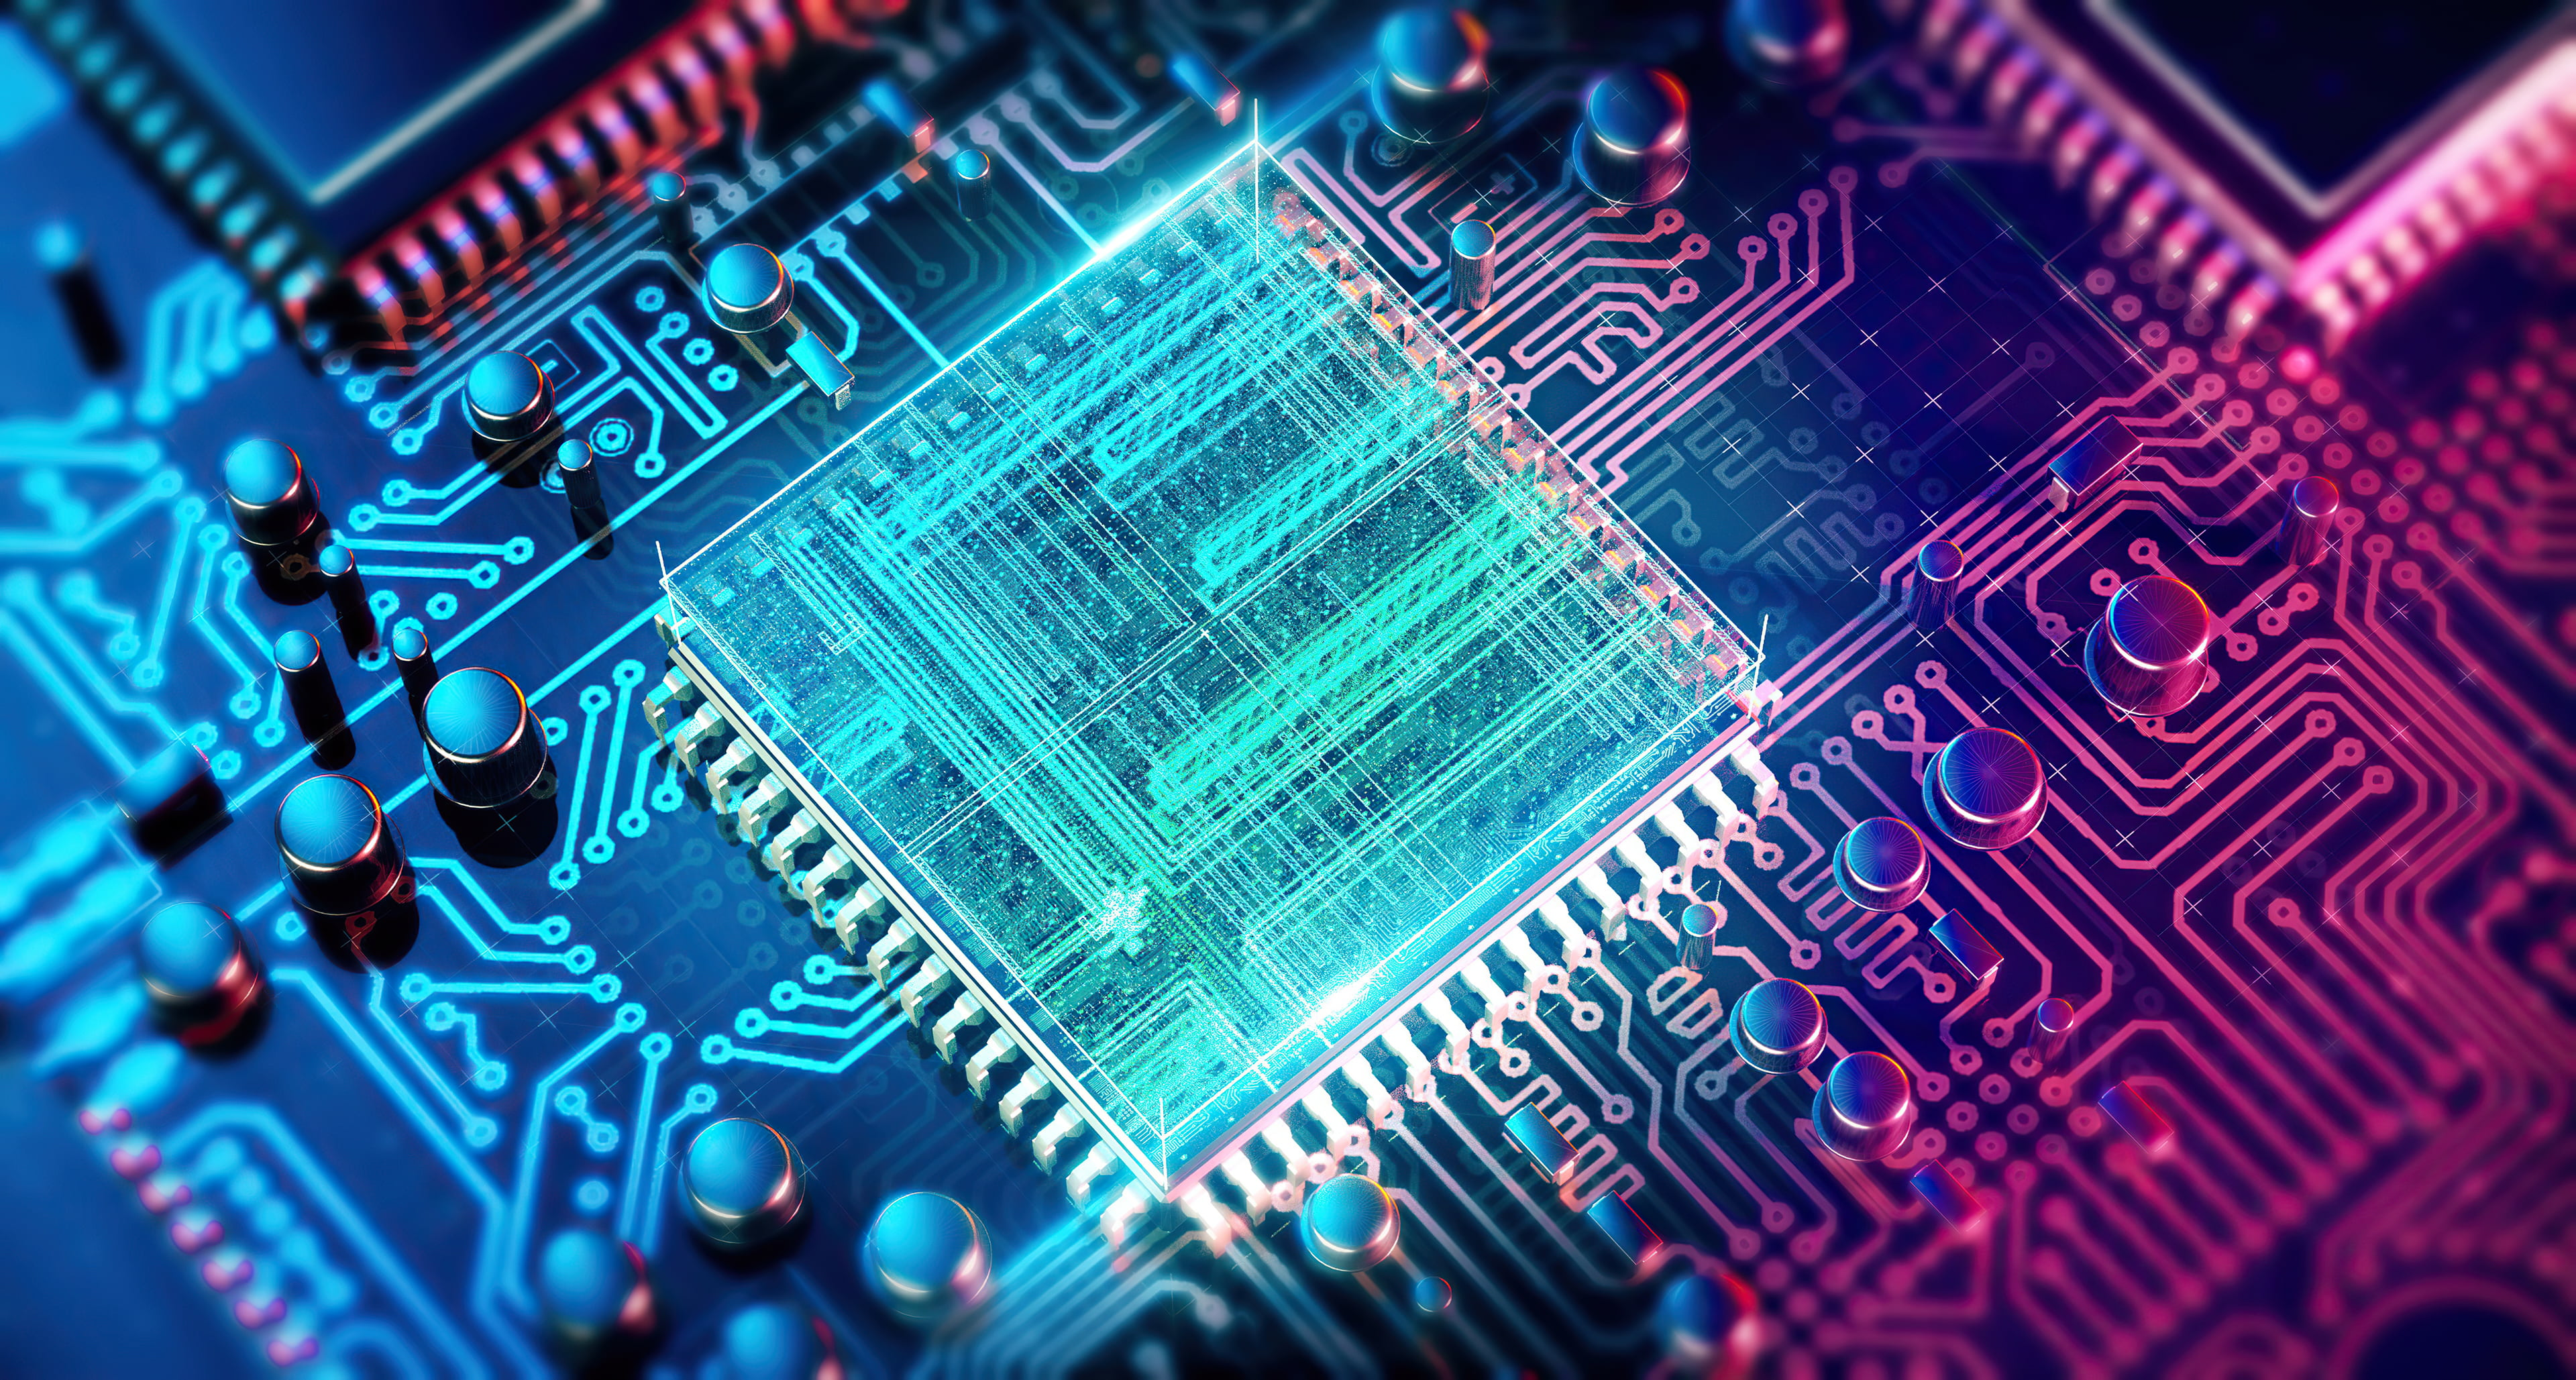
\includegraphics[height=\paperheight]{title.jpg}}

\def\subsectionname{}

% enumerate global settings
\setlist[enumerate,1]{label=\arabic*.}
\setlist[enumerate,2]{label=\alph*)}

% custom colors %
\definecolor{PolynesianBlue}{HTML}{0D519A}
\definecolor{MountbattenPink}{HTML}{997E9A}
\definecolor{RoyalBlue}{HTML}{0D266D}
\definecolor{HonoluluBlue}{HTML}{107EC0}
\definecolor{CoolGray}{HTML}{A4A4C1}

\colorlet{tPrim}{RoyalBlue}
\colorlet{tSec}{PolynesianBlue}
\colorlet{tAccent}{MountbattenPink}
\colorlet{tTheme}{RoyalBlue}
\colorlet{tTxt}{Black}

\tcbset{
 boxsep=7pt,
 fonttitle=\sc,
 colframe=tGreyBg,
 colframe=tTheme,
 boxrule=1pt
}

\begin{document}
\titleframe

\begin{frame}
 \frametitle{Obsah}
 \tableofcontents
\end{frame}

\section{Konečný automat a datová cesta}

\begin{frame}
 \frametitle{Konečný automat a datová cesta}
 \alert{Konečný automat} (angl. FSM -- finite-state machine) je výpočetní model
 v teoretické informatice. \pause
 Je to popis velmi jednoduchého počítače, který může být v jednom z několika
 stavů, mezi kterými přechází na základě informací ze vstupu.\\
 \pause
 \vspace{1em}
 \alert{Datová cesta} (angl. Datapath) je sdružení jednotek provádějících
 výpočetní operace, registrů a řadičů.
\end{frame}

\begin{frame}
 \frametitle{Příklad -- Faktoriál}
 Postavíme FSM, který umí spočítat $n! = n \cdot (n-1) \cdot (n-2) \cdot \ldots
 \cdot 2 \cdot 1$.\\
 \pause
 \vspace{\parskip}
 \begin{minipage}[t]{.45\textwidth}
  \begin{center}
   \textbf{V pseudokódu:}
   \begin{algorithm}[H]
    \SetKwProg{Dokud}{dokud}{ opakuj}{konec}
    $a = 1$\;
    $b = n$\;
    \Dokud{$b \neq 0$}{
     $a = a \cdot b$\;
     $b = b - 1$\;
    }
   \end{algorithm}
  \end{center}
 \end{minipage}
 \pause
 \begin{minipage}[t]{.45\textwidth}
  \begin{center}
   \textbf{Průběh pro $n = 5$:}\\
   \BlankLine
   \begin{tabular}{lll}
    na začátku: & $a = 1$ & $b = 5$\pause\\
    \midrule
    po 1. iteraci: & $a = 5$ & $b = 4$\\
    \pause
    po 2. iteraci: & $a = 20$ & $b = 3$\\
    \pause
    po 3. iteraci: & $a = 60$ & $b = 2$\\
    \pause
    po 4. iteraci: & $a = 120$ & $b = 1$\\
    \pause
    po 5. iteraci & $a = 120$ & $b = 0$\pause\\
    \midrule
    konec & & 
   \end{tabular}
  \end{center}
 \end{minipage}
\end{frame}

\begin{frame}
 \frametitle{Příklad -- Faktoriál}
 FSM vykonávající tento algoritmus:
 \vspace*{-\parskip}
 \begin{center}
  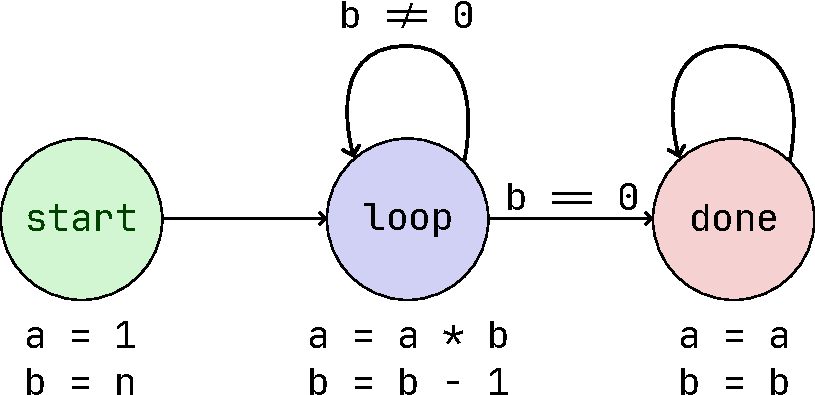
\includegraphics[width=.4\textwidth]{factorial.pdf}
 \end{center}
 \vspace*{-\parskip}
 \pause
 Pro převod do hardwarové podoby potřebujeme:
 \pause
 \begin{itemize}[label=\textbullet,topsep=0pt]
  \item dva registry -- pro $a$ a pro $b$,
  \pause
  \item dva bity pro uložení stavu -- start/loop/done,
  \pause
  \item logické přechody -- $b == 0$ a $b \neq 0$,
  \pause
  \item přiřazení hodnoty registrům -- $a = a \cdot b$ a $b = b - 1$.
 \end{itemize}
\end{frame}

\begin{frame}
 \frametitle{Datová cesta pro Faktoriál}
 Nejprve přidáme registry pro $a$ a $b$.
 \begin{center}
  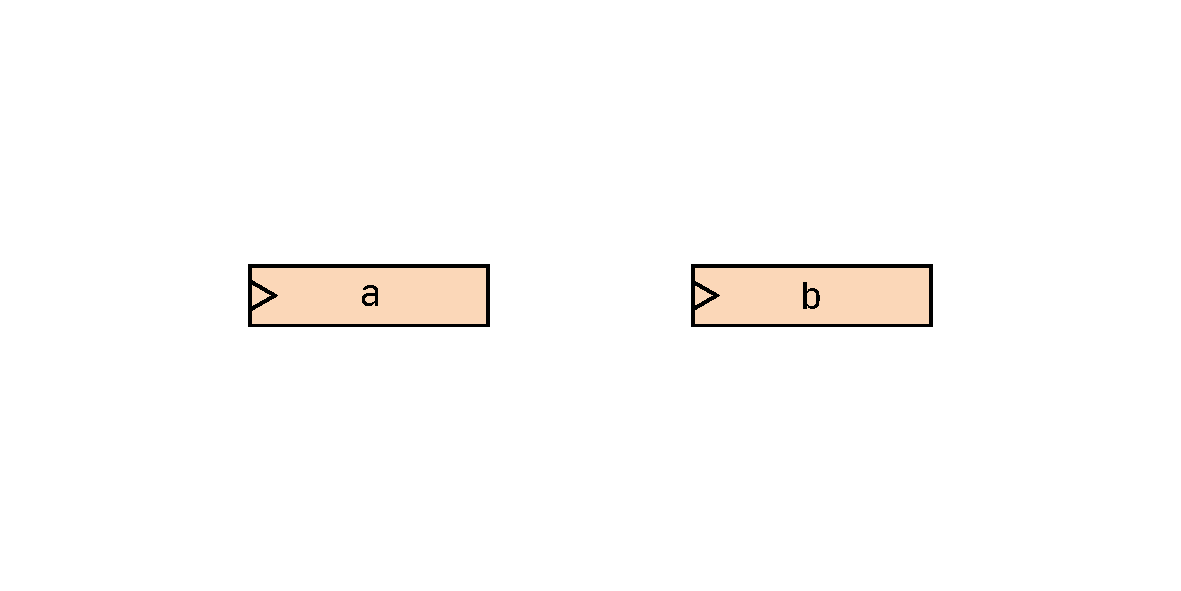
\includegraphics[width=.75\textwidth]{factorial-circuit-1.pdf}
 \end{center}
\end{frame}

\begin{frame}
 \frametitle{Datová cesta pro Faktoriál}
 Na začátku musejí registry obdržet hodnoty $1$ a $n$.
 \begin{center}
  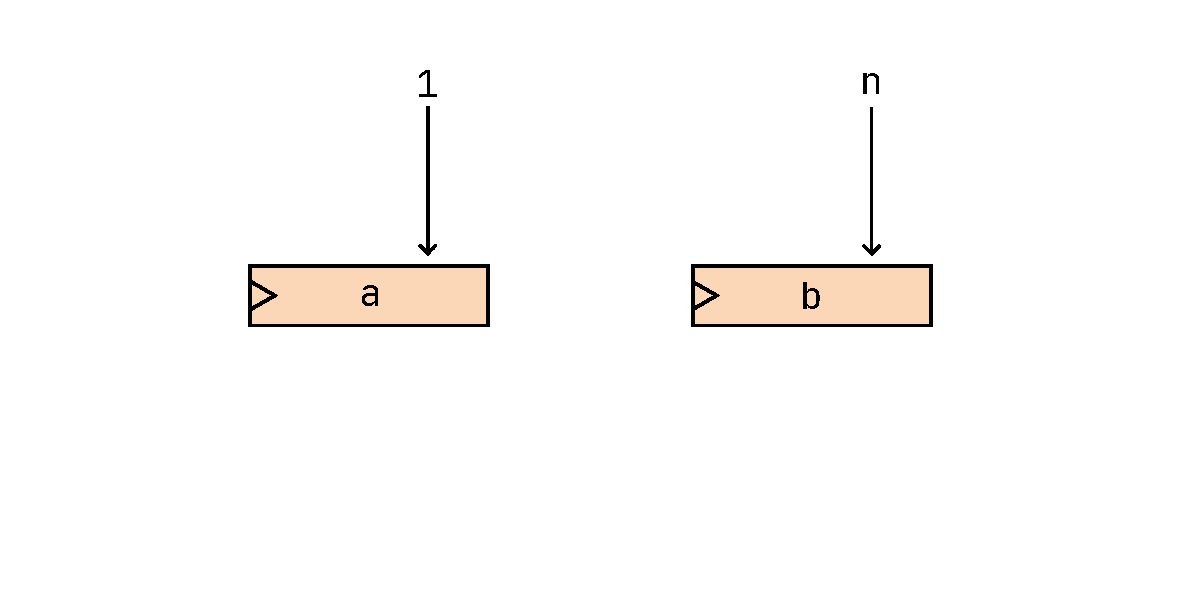
\includegraphics[width=.75\textwidth]{factorial-circuit-2.pdf}
 \end{center}
\end{frame}

\begin{frame}
 \frametitle{Datová cesta pro Faktoriál}
 Přidáme logický obvod pro násobení $a \cdot b$.
 \begin{center}
  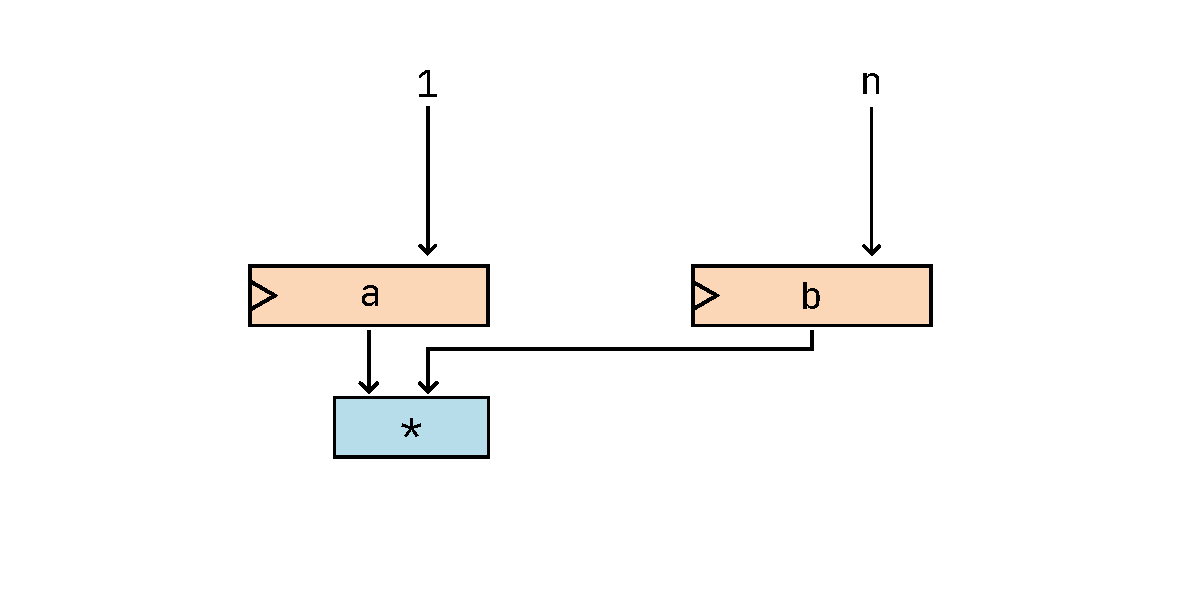
\includegraphics[width=.75\textwidth]{factorial-circuit-3.pdf}
 \end{center}
\end{frame}

\begin{frame}
 \frametitle{Datová cesta pro Faktoriál}
 Přidáme logický obvod pro součet $b + (-1)$.
 \begin{center}
  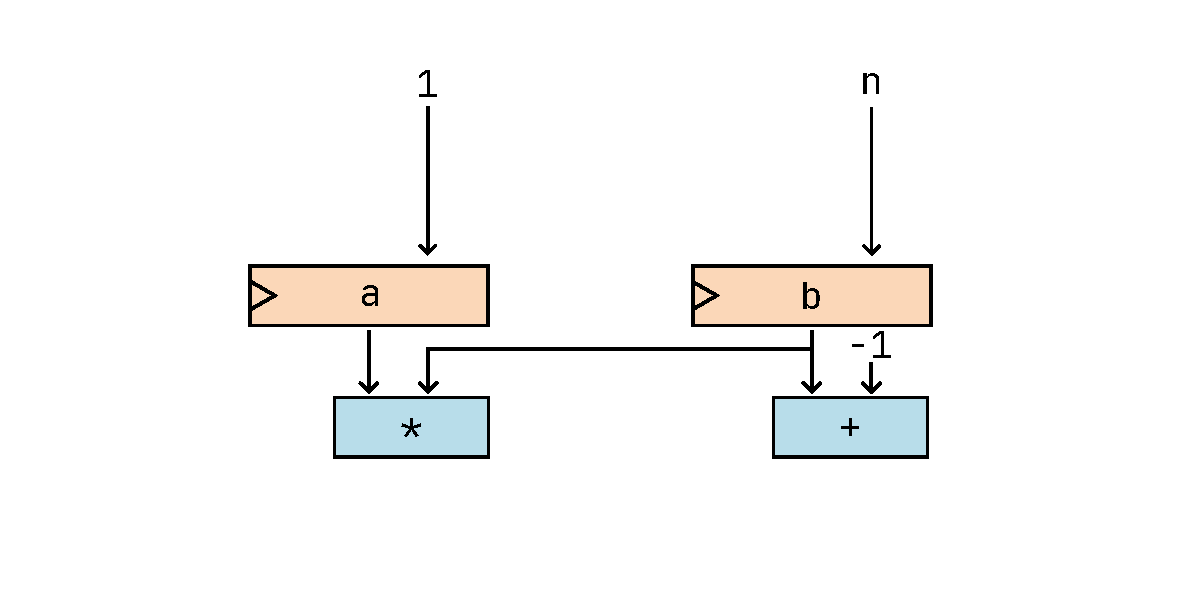
\includegraphics[width=.75\textwidth]{factorial-circuit-4.pdf}
 \end{center}
\end{frame}

\begin{frame}
 \frametitle{Datová cesta pro Faktoriál}
 Přidáme cestu zpět z výpočetních obvodů do registrů pro $a$ a $b$.
 \begin{center}
  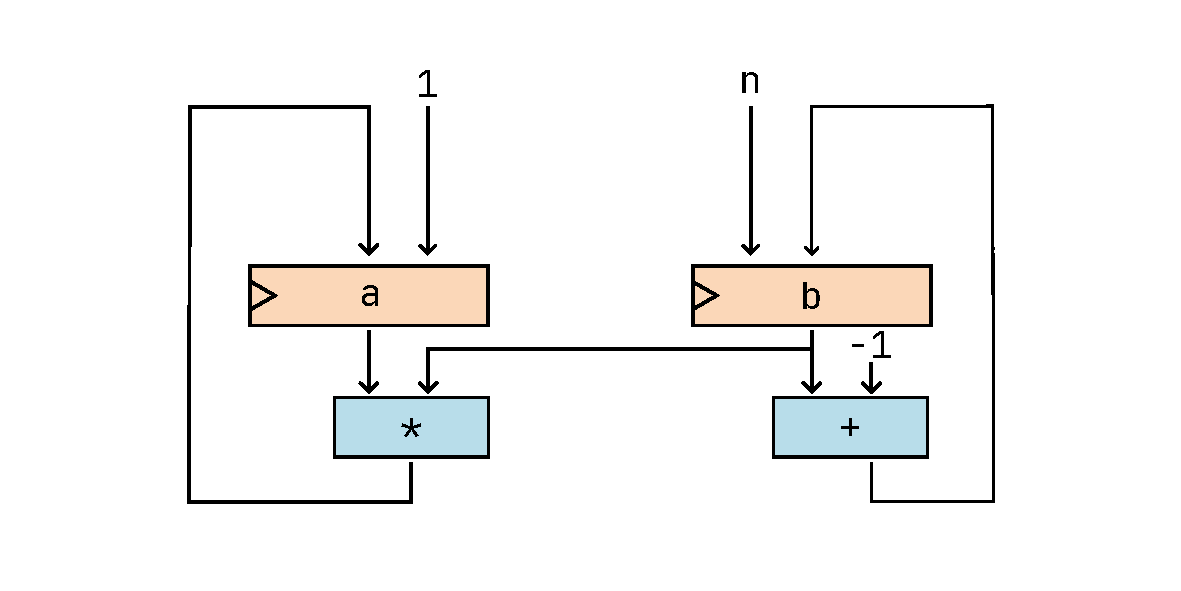
\includegraphics[width=.75\textwidth]{factorial-circuit-5.pdf}
 \end{center}
\end{frame}

\begin{frame}
 \frametitle{Datová cesta pro Faktoriál}
 Přidáme cestu z registrů pro $a$ a $b$ zpět do nich samých, aby po skončení
 výpočtu mohly uchovat informaci.
 \begin{center}
  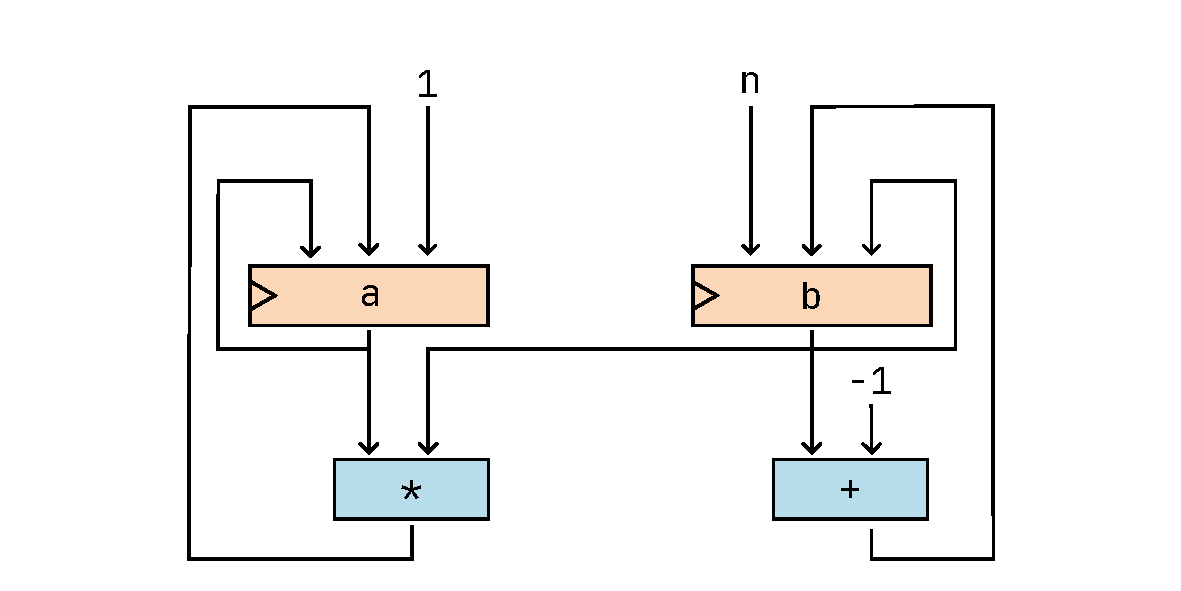
\includegraphics[width=.75\textwidth]{factorial-circuit-6.pdf}
 \end{center}
\end{frame}

\begin{frame}
 \frametitle{Datová cesta pro Faktoriál}
 Přidáme přepínače stavů, aby vždy do registrů pouštěly jen jeden vstup podle
 stavu výpočtu.
 \begin{center}
  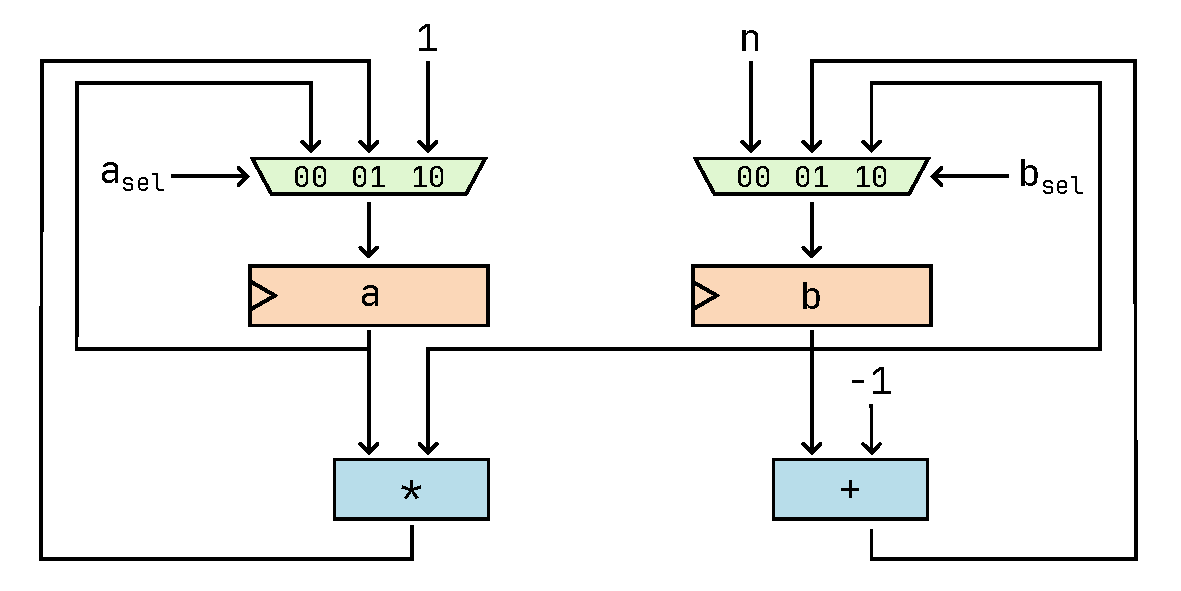
\includegraphics[width=.75\textwidth]{factorial-circuit-7.pdf}
 \end{center}
\end{frame}

\begin{frame}
 \frametitle{Řídící FSM pro Faktoriál}
 Přepínání vstupů do registrů pro $a$ a $b$ musí řídit nějaká jednotka --
 konečný automat.\pause\\
 Ta musí přepínat $a_{\text{sel}}$ a $b_{\text{sel}}$ během výpočtu.
 \begin{center}
  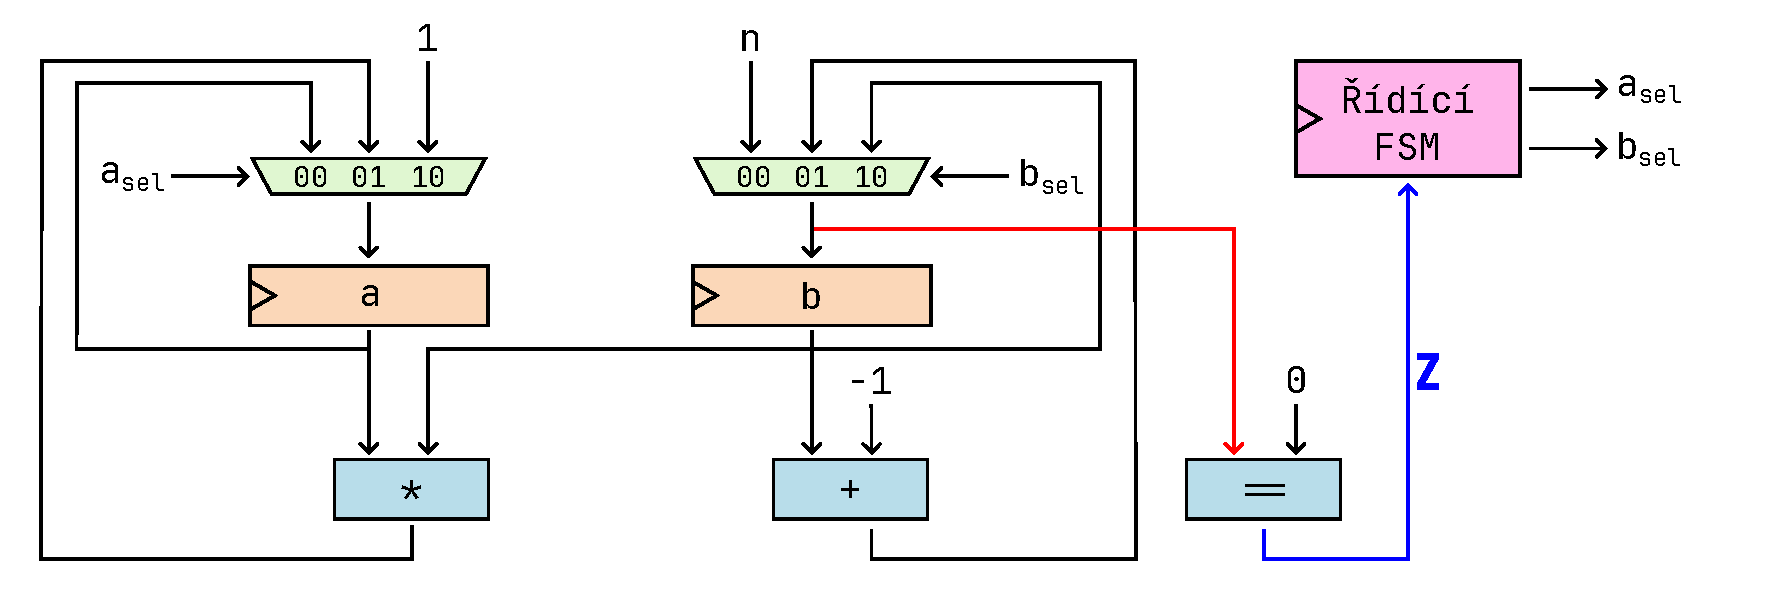
\includegraphics[width=\textwidth]{factorial-circuit-8.pdf}
 \end{center}
\end{frame}

\section{von Neumannův model}

\begin{frame}
 \frametitle{von Neumannův model}
 Nejpoužívanější model víceúčelového počítače. Skoro všechny moderní počítače
 jsou postaveny na tomto principu.
\end{frame}

\begin{frame}
 \frametitle{von Neumannův model}
 Nejpoužívanější model víceúčelového počítače. Skoro všechny moderní počítače
 jsou postaveny na tomto principu.\\
 Komponenty:
 \vspace*{-1em}
 \begin{center}
  
\includegraphics[width=.75\textwidth]{von-neumann-1.pdf}
 \end{center}
 \begin{itemize}[label=\textbullet]
  \item \alert{CPU}: Provádí aritmetické a logické operace na datech uložených v
   paměti a registrech.
 \end{itemize}
\end{frame}

\begin{frame}
 \frametitle{von Neumannův model}
 Nejpoužívanější model víceúčelového počítače. Skoro všechny moderní počítače
 jsou postaveny na tomto principu.\\
 Komponenty:
 \vspace*{-1em}
 \begin{center}
  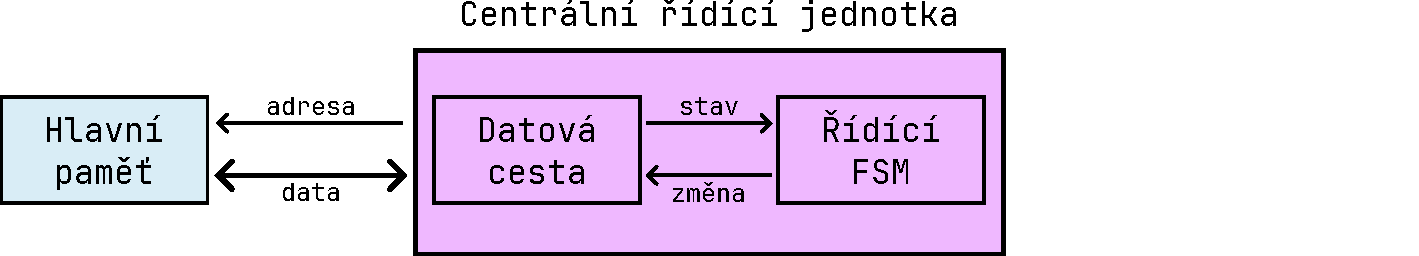
\includegraphics[width=.75\textwidth]{von-neumann-2.pdf}
 \end{center}
 \begin{itemize}[label=\textbullet]
  \item \alert{CPU}: Provádí aritmetické a logické operace na datech uložených v
   paměti a registrech.
  \item \alert{Hlavní (dnes \uv{vnitřní}) paměť}: Seznam \alert{slov} o daném
   počtu \alert{bitů} 
 \end{itemize}
\end{frame}

\begin{frame}
 \frametitle{von Neumannův model}
 Nejpoužívanější model víceúčelového počítače. Skoro všechny moderní počítače
 jsou postaveny na tomto principu.\\
 Komponenty:
 \vspace*{-1em}
 \begin{center}
  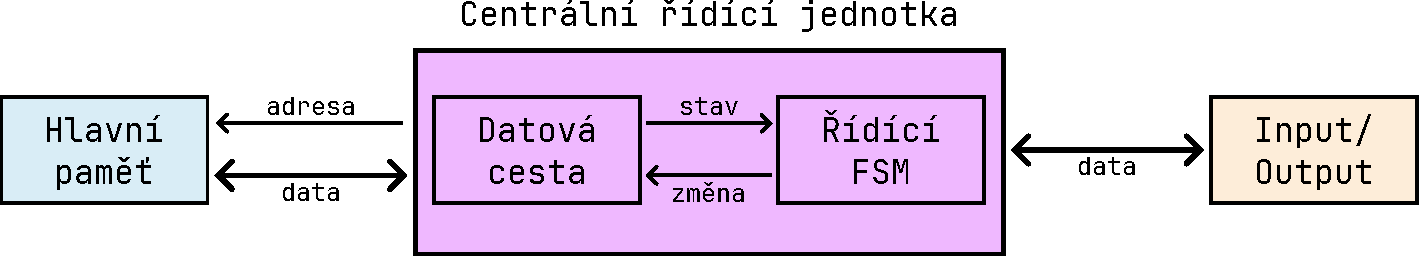
\includegraphics[width=.75\textwidth]{von-neumann-3.pdf}
 \end{center}
 \begin{itemize}[label=\textbullet]
  \item \alert{CPU}: Provádí aritmetické a logické operace na datech uložených v
   paměti a registrech.
  \item \alert{Hlavní (dnes \uv{vnitřní}) paměť}: Seznam \alert{slov} o daném
   počtu \alert{bitů}.
  \item \alert{Input/output}: Libovolná zařízení umožňující interakci s vnějším
   světem.
 \end{itemize}
\end{frame}

\begin{frame}
 \frametitle{Klíčová idea: program uložený v hlavní paměti}
 \begin{itemize}[label=\textbullet]
  \item Vyjádření programu jako posloupnosti zakódovaných instrukcí.\pause
  \item Paměť ukládá \alert{jak program, tak instrukce!}\pause
  \item CPU \alert{vyzvedne, přeloží} a \alert{vykoná} (fetch-decode-execute
   cyklus) instrukce programu, jak jdou za sebou.
 \end{itemize}
\end{frame}

\begin{frame}
 \frametitle{Klíčová idea: program uložený v hlavní paměti}
 \vspace*{-1em}
 \begin{center}
  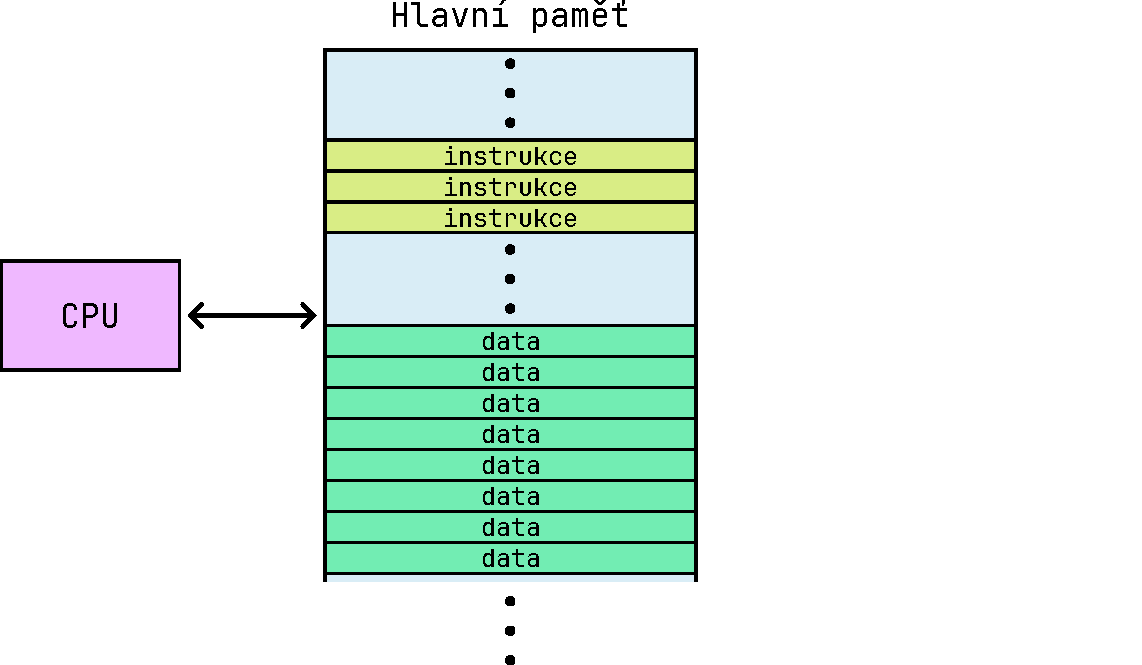
\includegraphics[width=.5\textwidth]{instructions-1.pdf}
 \end{center}
\end{frame}

\begin{frame}
 \frametitle{Klíčová idea: program uložený v hlavní paměti}
 \begin{center}
  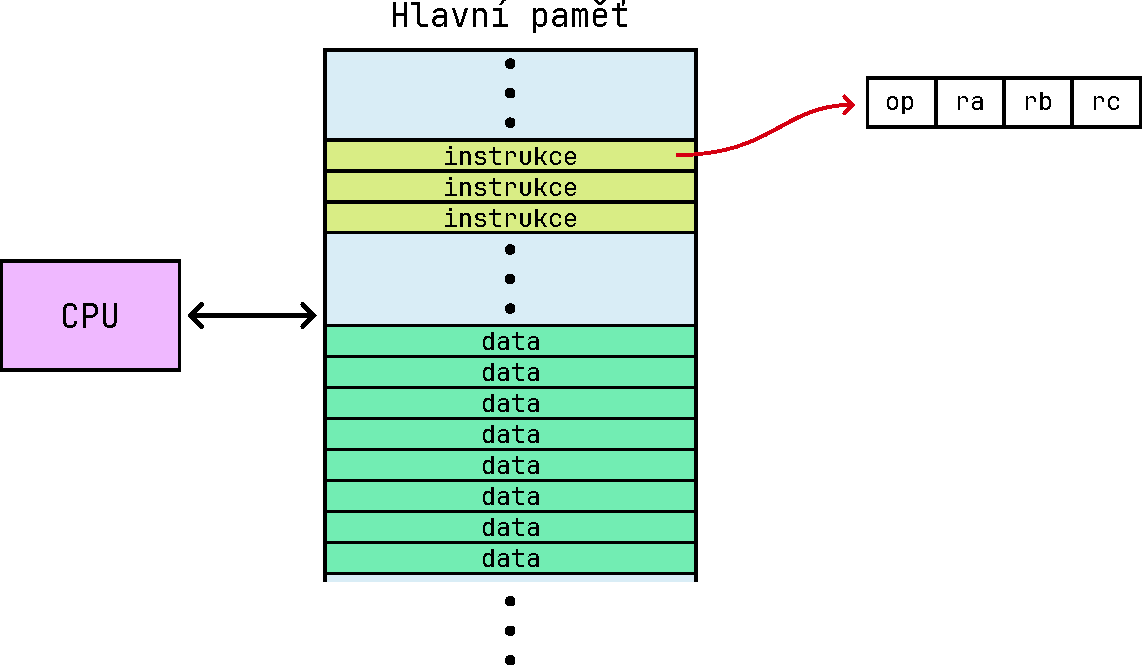
\includegraphics[width=.5\textwidth]{instructions-2.pdf}
 \end{center}
 \vspace*{-3em}
 \begin{itemize}[label=\textbullet]
  \item \alert{Instrukce} je obvykle čtveřice
  \begin{itemize}[label=\textemdash]
   \item operace (\texttt{op}),
   \item registr s prvním operandem (\texttt{ra}),
   \item registr s druhým operandem (\texttt{rb}),
   \item registr pro uložení výsledku (\texttt{rc}).
  \end{itemize}
 \end{itemize}
\end{frame}

\begin{frame}
 \frametitle{Klíčová idea: program uložený v hlavní paměti}
 \begin{center}
  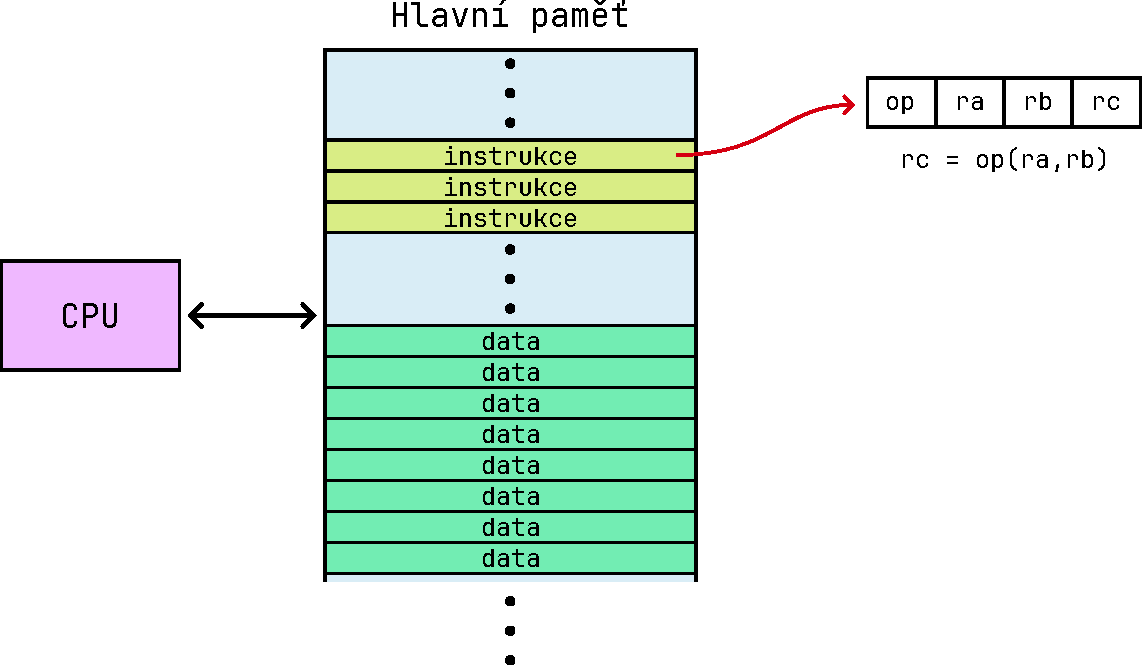
\includegraphics[width=.5\textwidth]{instructions-3.pdf}
 \end{center}
 \vspace*{-1em}
 \begin{itemize}[label=\textbullet]
  \item CPU tuhle instrukci přeloží jako, \uv{Proveď \texttt{op} na hodnotu v
   \texttt{ra} a hodnotu v \texttt{rb} a výsledek ulož do \texttt{rc}}.
 \end{itemize}
\end{frame}

\begin{frame}
 \frametitle{Klíčová idea: program uložený v hlavní paměti}
 \begin{center}
  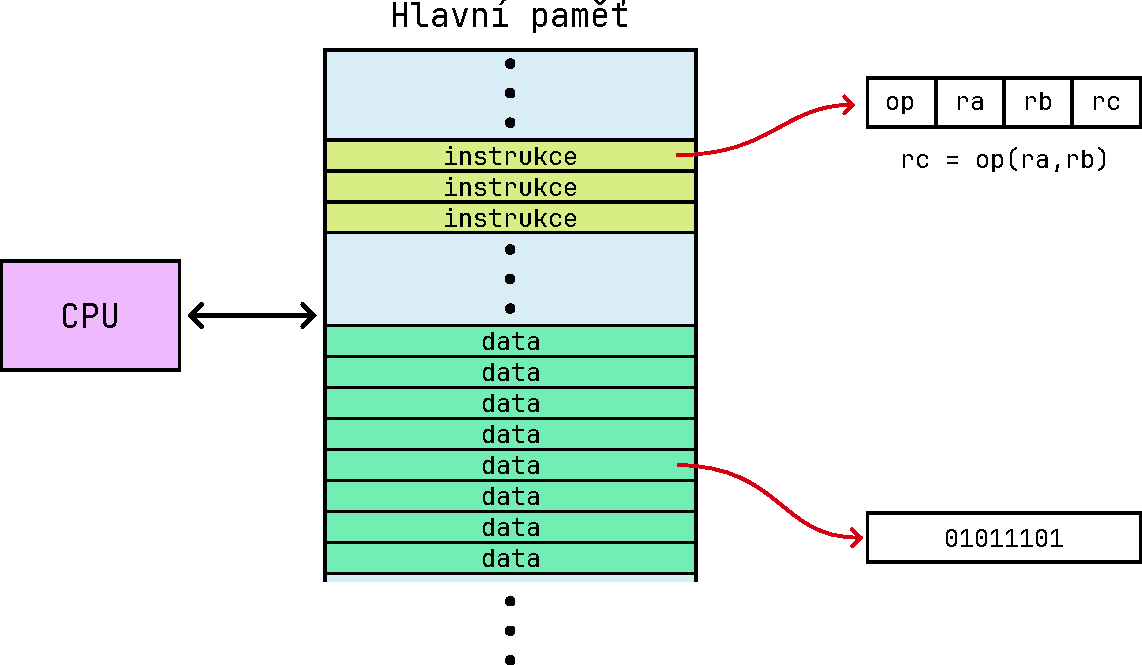
\includegraphics[width=.5\textwidth]{instructions-4.pdf}
 \end{center}
 \vspace*{-1em}
 \begin{itemize}[label=\textbullet]
  \item Bloky (řádky) paměti s daty nemají žádný daný formát. Jsou to zkrátka
   jen uložené hodnoty vzniklé nějakým výpočtem v minulosti. Mohou to být slova,
   čísla či cokoli jiného.
  \pause
  \item Každý blok má daný počet bitů (v tomto příkladě 8).
 \end{itemize}
\end{frame}

\begin{frame}
 \frametitle{Klíčová idea: program uložený v hlavní paměti}
 \alert{Problém:} Jak poznám, co je instrukce a co datum?\pause\\
 \begin{itemize}[label=\textbullet]
  \item Pamatujte, že CPU i paměť jsou pořád jenom logické (elektrické)
   obvody.\pause
  \item To znamená, že je možné ukládat instrukce tak, aby šly přímo do
   \alert{řídící FSM} a data naopak přímo do \alert{datové cesty (a tam do
   registrů)}.\pause
  \item CPU je pak navržen tak, že posloupnost bitů v řídící FSM považuje za
   instrukci, zatímco v datové cestě za datum.
 \end{itemize}
\end{frame}

\begin{frame}
 \frametitle{Anatomie von Neumannova počítače}
 \begin{columns}[T]
  \begin{column}{.6\textwidth}
   \vspace*{-1em}
   \begin{center}
    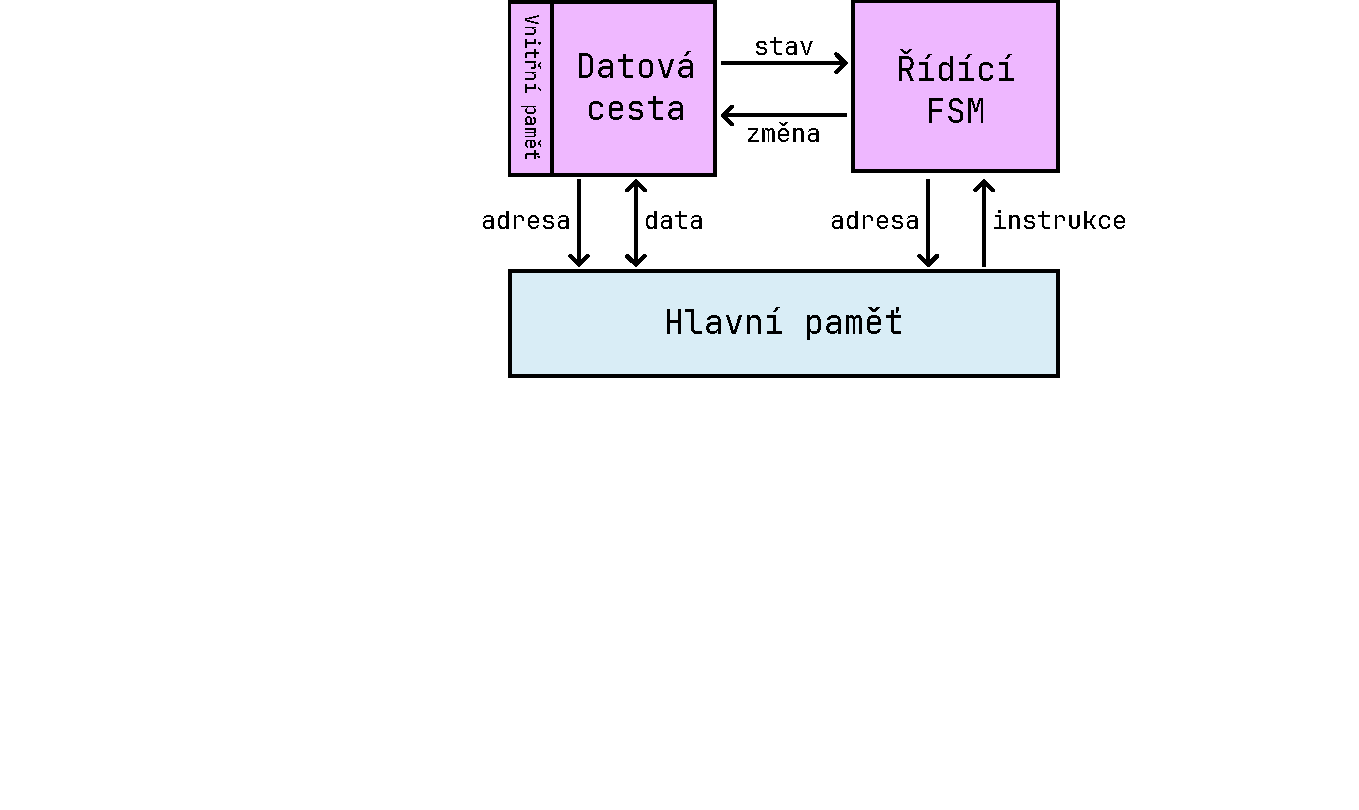
\includegraphics[width=1.2\textwidth]{anatomy-1.pdf}
   \end{center}
  \end{column}
  \begin{column}{.39\textwidth}
  \end{column}
 \end{columns}
\end{frame}

\begin{frame}
 \frametitle{Anatomie von Neumannova počítače}
 \begin{columns}[T]
  \begin{column}{.6\textwidth}
   \vspace*{-1em}
   \begin{center}
    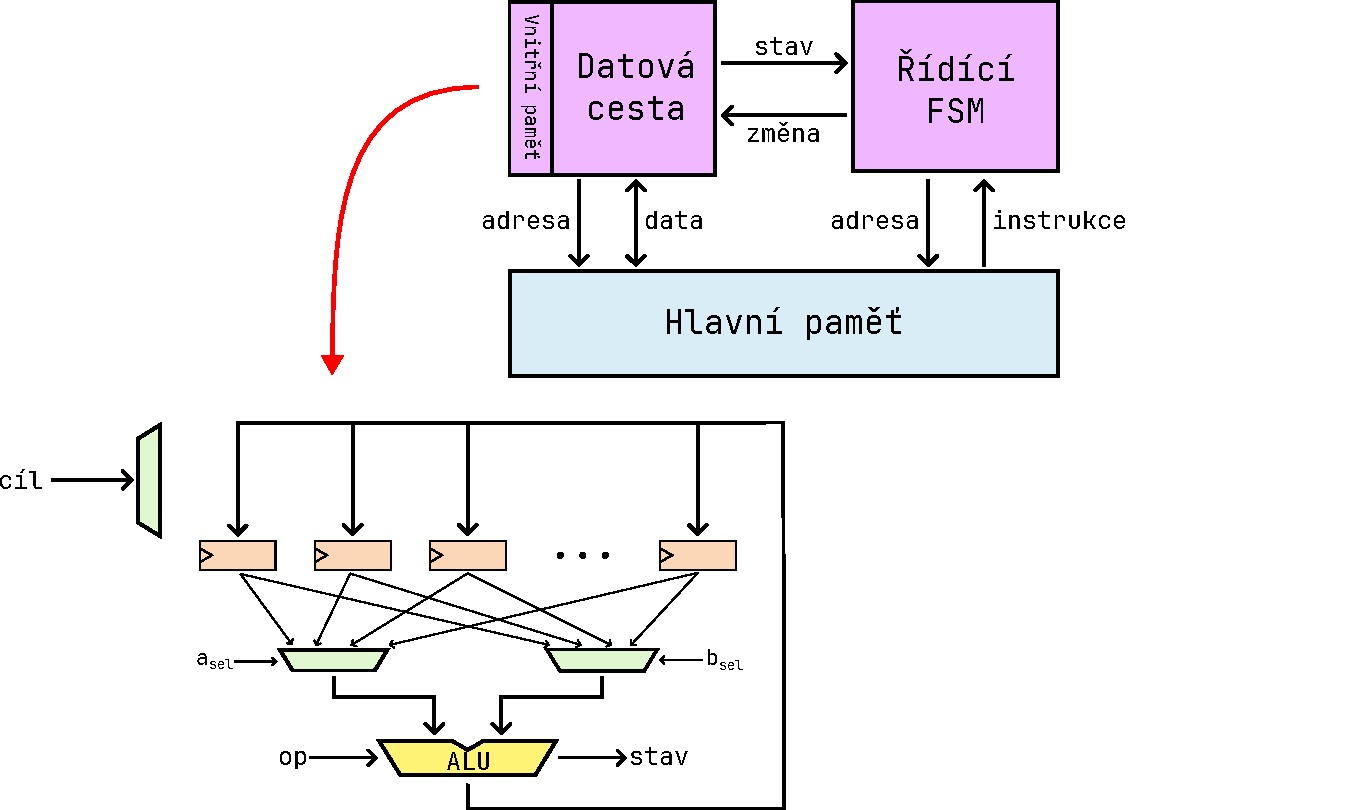
\includegraphics[width=1.2\textwidth]{anatomy-2.pdf}
   \end{center}
  \end{column}
  \begin{column}{.39\textwidth}
  \end{column}
 \end{columns}
\end{frame}

\begin{frame}
 \frametitle{Anatomie von Neumannova počítače}
 \begin{columns}[T]
  \begin{column}{.6\textwidth}
   \vspace*{-1em}
   \begin{center}
    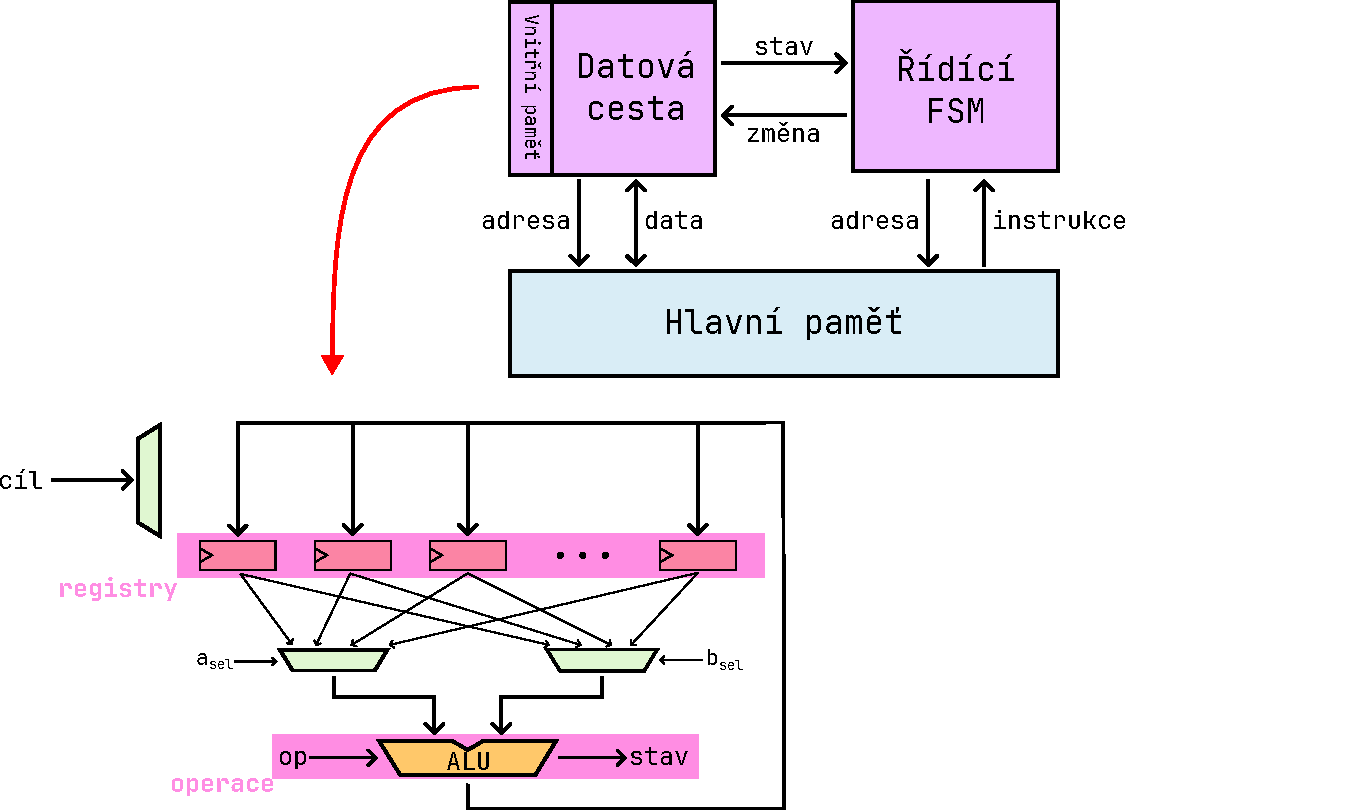
\includegraphics[width=1.2\textwidth]{anatomy-3.pdf}
   \end{center}
  \end{column}
  \begin{column}{.39\textwidth}
  \end{column}
 \end{columns}
\end{frame}

\begin{frame}

 \frametitle{Anatomie von Neumannova počítače}
 \begin{columns}[T]
  \begin{column}{.6\textwidth}
   \vspace*{-1em}
   \begin{center}
    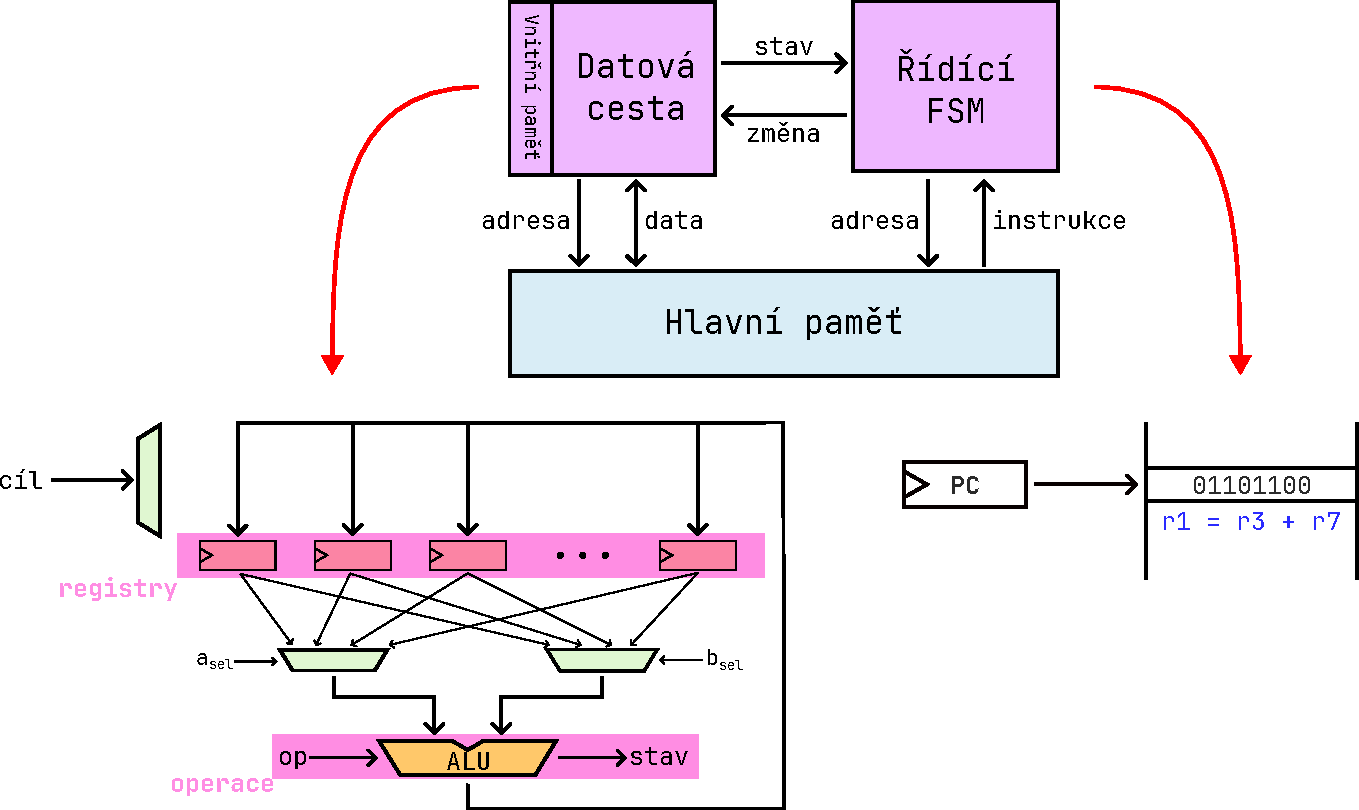
\includegraphics[width=1.2\textwidth]{anatomy-4.pdf}
   \end{center}
  \end{column}
  \begin{column}{.39\textwidth}
   \begin{itemize}[label=\textbullet]
    \item \alert{Instrukce} zakódovány jako binární čísla.\pause
    \item \alert{Čítač} (PC -- Program Counter): adresa instrukce, která se má
     vykonat.\pause
   \end{itemize}
   \vspace{3em}
   \begin{itemize}[label=\textbullet]
    \item Postup pro překlad instrukcí do signálů pro datovou cestu.
   \end{itemize}
  \end{column}
 \end{columns}
\end{frame}

\begin{frame}
 \frametitle{Anatomie von Neumannova počítače -- Instrukce}
 \begin{itemize}[label=\textbullet]
  \item Instrukce jsou základní jednotkou práce.\pause
  \item Každá instrukce specifikuje
  \begin{itemize}[label=\textemdash]
   \item \alert{operaci}, která se má vykonat,\pause
   \item registry se zdrojovými \alert{operandy} a \alert{cílový registr} pro
    výsledek.
  \end{itemize}
  \begin{columns}[T]
   \begin{column}{.65\textwidth}
    \begin{itemize}[label=\textbullet]
     \item Ve von Neumannově počítači jsou instrukce čteny postupně
     \pause
     \begin{itemize}[label=\textemdash]
      \item CPU implementuje cyklus napravo:
      \item Pokud právě vykonaná instrukce nespecifikuje jinak, je adresa další
       instrukce v pořadí adresa této + délka instrukce (v bitech).
     \end{itemize}
    \end{itemize}
   \end{column}
   \begin{column}{.29\textwidth}
    \begin{center}
     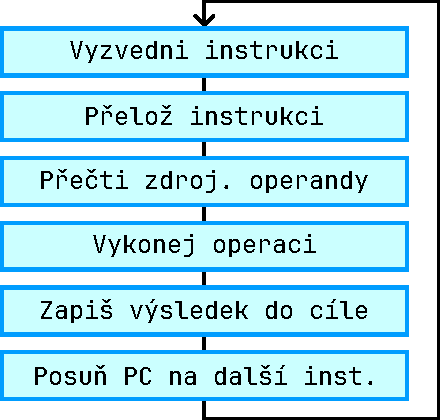
\includegraphics[width=\textwidth]{instruction-reading.pdf}
    \end{center}
   \end{column}
  \end{columns}
 \end{itemize}
\end{frame}

\section{Architektura instrukční sady}

\begin{frame}
 \frametitle{Architektura instrukční sady}
 Architektura instrukční sady (angl. \alert{ISA} -- Instruction Set
 Architecture) je jakási \uv{dohoda} mezi softwarem a hardwarem.\pause\\
 \begin{itemize}[label=\textbullet]
  \item \alert{Software} jsou programy uložené ve vnitřní paměti -- dají se
   měnit.\pause
  \item \alert{Hardware} jsou logické obvody tvořící počítač -- nelze je
   měnit.\pause
  \item \alert{ISA} obsahuje
  \begin{itemize}[label=\textemdash]
   \item definice \alert{operací} a \alert{adres pro ukládání},\pause
   \item \alert{přesný popis} toho, jak je software má \alert{nařídit} a
    \alert{dostat se k nim}.
  \end{itemize}
 \end{itemize}
\end{frame}

\begin{frame}
 \frametitle{Architektura instrukční sady}
 ISA je další úroveň abstrakce umožňující vývoj hardware \alert{bez ohledu na
 software}.\pause
 \begin{itemize}[label=\textbullet]
  \item ISA specifikuje, \alert{co} hardware poskytuje, nikoli \alert{jak}
   (nespecifikuje implementaci logických obvodů v CPU).\pause
  \item Dokud je ISA dodržena, je možné vylepšovat hardware zcela bez ohledu na
   software, který ho používá. Např.
  \begin{itemize}[label=\textemdash]
   \item Intel 8086 (z roku 1978) má 29 tisíc tranzistorů, hodiny s frekvencí 5
    MHz a zvládne asi 330 tisíc operací za sekundu;\pause 
   \item Intel Pentium 4 (2003) má 44 milionů tranzistorů, hodiny s frekvencí 4
    Ghz a zvládne asi 5 miliard operací za sekundu;\pause
  \end{itemize}
  oba procesory používají instrukční sadu x86.
 \end{itemize}
\end{frame}

\begin{frame}
 \frametitle{Architektura instrukční sady}
 Navrhnout ISA je obtížné.
 \begin{itemize}[label=\textbullet]
  \item Kolik operací a jaké?\pause
  \item Jaké typy úložišť? Kolik?\pause
  \item Jak kódovat instrukce?\pause
  \item Jak zařídit kompatibilitu s budoucím hardwarem?\pause
 \end{itemize}
 \alert{Statistický přístup:}
 \begin{itemize}[label=\textbullet]
  \item Vybere se mnoho testovacích programů.\pause
  \item Každá verze ISA se otestuje na každém programu.\pause
  \item Určí se nejběžněji používané operace -- rychlost jejich provedení a
   spotřeba energie se optimalizuje.
 \end{itemize}
\end{frame}

\end{document}
